\section{Introduction}
\label{sec:intro}

% maybe put this in a figure.tex
\newcommand{\architectureoverview}{
    \begin{figure*}[ht]
    \centering
    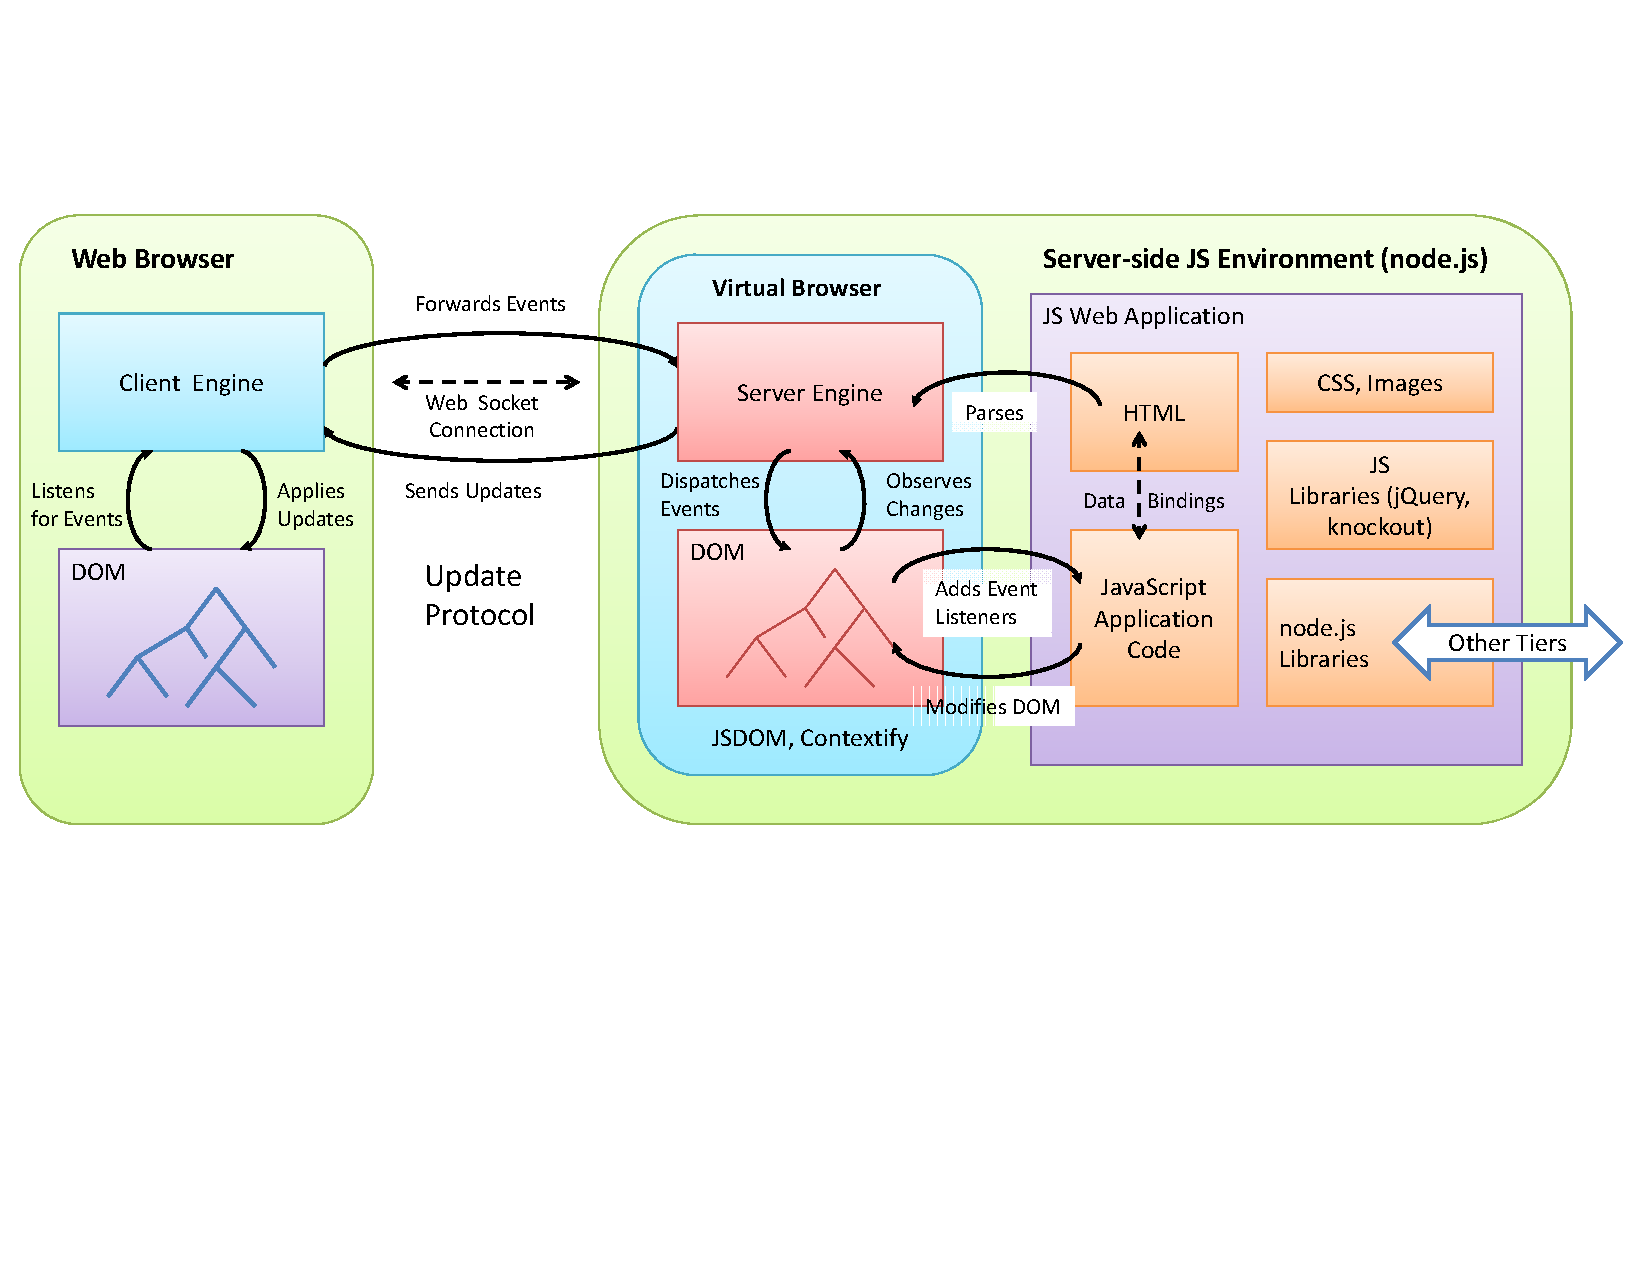
\includegraphics[width=\textwidth]{figs/architecture_overview.pdf}
    \caption{Single Process \cb{} Architecture Overview}
    \label{fig:cb1arch}
    \end{figure*}
}

% backgroud, motivation, design choices, architecture , experiments(goals, etc.)
Before AJAX~\cite{garrett2005ajax} became pervasive, a typical web application works like this:
the user sends a request to the web server by submitting a form or clicking a link on a web page,
then the server processes this request and responds with a new HTML document.
The problem about this form/link based model is that it is hard
to create responsive and rich user experience because the whole user interface
is wiped out and re-rendered every time user sends a request.

AJAX is an approach that uses javascript to send requests to server
and partially updates the HTML document without page refresh.
It is capable of delivering a better performance and native application like user experience.
In this model, developers have to write client javascript code to handle server client communication
and rendering logic.


\cb{} is a server-centric framework designed to simplify the development of AJAX web applications.
Developer's code is running in a server side virtual browser and the user's browser is just
a dumb display device which synchronizes with the virtual browser.
In \cb{}, developers use nothing but HTML, css and javascript to construct the UI logic just like
any traditional AJAX application.
In the place where traditional AJAX applications call a server side API through HTTP,
developers could call a server side method directly.
The view synchronization between the virtual browser and the actual browser is 
handled by the framework under the hood.
\cb{} also naturally preserves UI state upon page refreshes
because all the UI state is kept in the server side.


%Comparing to other server-centric frameworks, 
%\cb{} could reuse most of existing client code because it does not require an extra markup language
%and its sole programming language is javascript.

Fig.\ref{fig:cb1arch} demonstrates the architecture of the original \cb{}. %FIXME expand in detail here
For a stateless web application,
scaling up would be accomplished by adding more processes and configuring the new processes
in a front end load balancer which distributes the client requests among all the processes.
However, for \cb{} it is vital to make sure the web server connects to the corresponding
virtual browser instance inside a particular process to get the right view state.
In the original \cb{}'s design, a \cb{} process contains all the virtual browsers.% FIXME
%It cannot benefit from multiple processors and provides no isolation between virtual browsers.
It is challenging to make a stateful application like \cb{} to support multiple process, 
but we think it is an effort worth taking :
the new design would boost \cb{}'s capacity to make it support larger scale web applications,
the process of implementing it also shed some light on how to scale Node.js applications in general.

\subsection{The architecture of the original \cb{}}
\cb{} is built using Node.js javascript execution environment. %FIXME
As shown in Fig.\ref{fig:cb1arch}, 
The user's browser will download the client engine written in javascript.
The client engine then connect to the server and fetch DOM elements in a
virtual browser
will connect to a virtual browser in server side and fetch DOM
elements from the 

The requests are translated to DOM events by the framework to be triggered on virtual browsers.
The application javascript code would handle these events and update the DOM elements.
Finally the 

% move this until you have the desired placement
\architectureoverview{} 

